%%%%%%%%%%%%%%%%%%%%%%%%%%%%%%%%%%%%%%%%%%%%%
% Standard projektübergreifender Header für
% - Makros 
% - Farben
% - Mathematische Operatoren
%
% DORT NUR ERGÄNZEN, NICHTS LÖSCHEN
%%%%%%%%%%%%%%%%%%%%%%%%%%%%%%%%%%%%%%%%%%%%%
\documentclass{article}
\input{header/zusammenfassung}
\input{header/hyperref}
\input{header/listings}

\usepackage{graphicx}		% Grafiken
\usepackage{color}			% Farben
\usepackage{lastpage}		% Seite x von y
\newcommand{\hoch}{$^{\wedge}$}


\title{Matlab Befehlsreferenz}
\author{Philipp Kälin, Hannes Badertscher}

%%%%%%%%%%%%
% Dokument %
%%%%%%%%%%%%
\begin{document}
  \def\thickhrulefill{\leavevmode \leaders \hrule height 1pt\hfill \kern \z@}

\begin{titlepage}
    \vspace{10cm} %\par
    \hrule height 4pt
    \begin{flushleft}
      \huge Matlab Befehlsreferenz
    \end{flushleft}
    \hrule height 4pt
    \par
    \begin{flushright}
      \begin{tabular}{r}
        \LARGE Philipp Kälin, Hannes Badertscher \\
        \hspace{1mm} \\
        \LARGE Version vom \today
      \end{tabular}
    \end{flushright}
    
    \vfill
      \begin{center}
        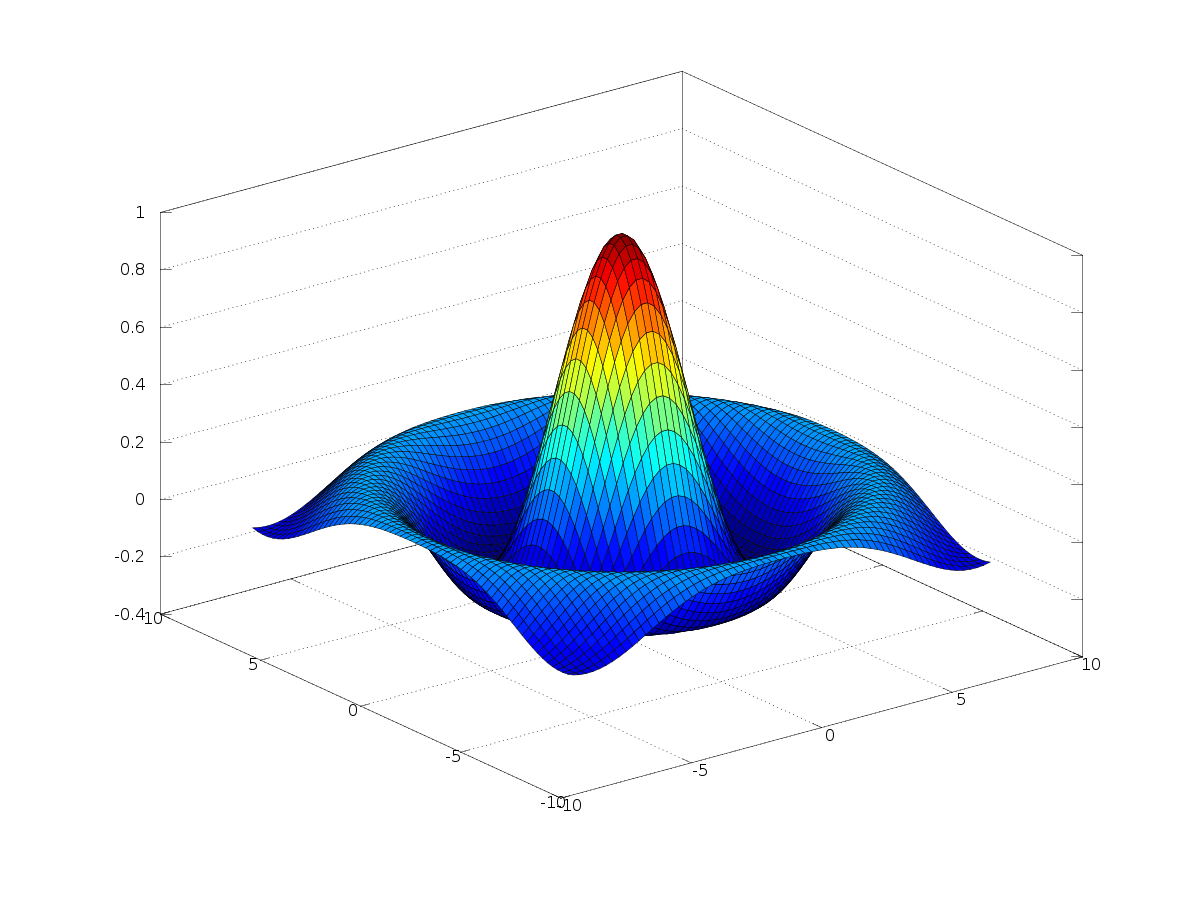
\includegraphics[width=20cm]{images/lorenz.png}
      \end{center}
    \vfill
    
    \hrule height 1.75pt \vspace{1mm}
    This work is licensed under a \newline
    \begin{tabular}{ll}
        \multirow{3}{*}{\includegraphics[height=1cm]{header/lizenzen/cc-by-nc-sa/small.png}} &
        %\mulrirow{2}{*}{} &
        \textit{Creative Commons Attribution-NonCommercial-ShareAlike 3.0
        Unported License.}
      \\
        &
        \url{http://creativecommons.org/licenses/by-nc-sa/3.0/}
      \\
      	&     \textit{powered by \LaTeX}
    \end{tabular}\\
    
\end{titlepage}%
\setcounter{footnote}{0}%

\section{Systemspezifische Befehle}
	\begin{tabularx}{\textwidth}{X|X}
  \begin{tabular}{ll}
      \multicolumn{2}{l}{\textbf{Befehle}}
    \\
      \texttt{clc}      & Commandfenster löschen
    \\
  		\texttt{clear}    &	Alle Variabelnzuweisungen löschen
  	\\
  	  \texttt{help}     & Hilfe zu einer Funktion
  	\\
      \texttt{load}     & Variabelnzuweisung wieder laden
    \\
      \texttt{lookfor}  & Befehle nach einem Suchbegriff durchsuchen
    \\
      \texttt{save}     & Alle Variabelnzuweisungen speichern
    \\
      \texttt{what}     & Dateien im aktuellen Verzeichnis anzeigen
    \\
      \texttt{whos}     & Verwendete Variabeln anzeigen
    \\
      \texttt{;}        & Befehl ausführen ohne anzuzeigen
    \\
      \texttt{simplify( )} & Ausdruck vereinfachen
    \\
      \texttt{pretty( )}   & Ausdruck in lesbarer Form anzeigen
    \\
      \texttt{grid on}  & Gitterlinien in einem Diagramm anzeigen
  \end{tabular}
  
& %--------------------------------------------------------------

  \begin{tabular}{ll}
    \multicolumn{2}{l}{\textbf{Operatoren}}
    \\
      \texttt{*}        & Matrix Multiplikation
    \\
      \texttt{.*}       & Array Multiplikation
    \\
      \texttt{./}       & Array Division
    \\
      \texttt{\hoch}    & Matrix Exponent
    \\
      \texttt{.\hoch}   & Array Exponene
    \\
      \texttt{'}        & Transponiert (mit konjugiert komplexen Zahlen)
    \\
      \texttt{.'}       & Transponiert (ohne Veränderung der komplexen Zahlen)
    \\
      \texttt{\textbackslash} & Lösung eines linearen Gleichungssystems
  \end{tabular}
  
\\
  \begin{tabular}{ll}
    \multicolumn{2}{l}{\textbf{Variabeln}}
    \\
      \texttt{ans}      & Letztes Resultat
    \\
      \texttt{pi}       & $\pi$
    \\
      \texttt{i, j}     & Imaginäre Einheit
  \end{tabular}
  
  & %---------------------------------------------------------------------
  \begin{tabular}{ll}
    \multicolumn{2}{l}{\textbf{Diverse}}
    \\
      \texttt{rand(x)}     & Zufallszahlen zwischen 0 und 1 gleichverteilt
    \\
      \texttt{randn(x)}    & Zufallszahlen um 0 mit Gaussverteilung
  \end{tabular}
  
\end{tabularx}

\section{Funktionen}
  \subsection{Allgemeine Mathematische Funktionen}

\begin{tabular}{lll}
    \textbf{Symbol} & \textbf{Matlab} & \textbf{Beschreibung}
  \\
     $ ln(x)dx $ &
    \texttt{diff(log(x),x)} &
  \\
    $ |x| $ &
    \texttt{abs(x)} &
    Betrag
  \\
    &
    \texttt{angle(x)} &
    Argument, Phase
  \\
    &  
    \texttt{ceil(x)} & 
    Runden (grösser oder gleich) zur nächsten Zahl
  \\
    &
    \texttt{floor(x)} &
    Runden (kleiner oder gleich) zur nächsten Zahl
  \\
    &
    \texttt{round(x)} &
    Rundung zur nächsten ganzen Zahl 
  \\
    &
    \texttt{conj(x)} &
    Konjugiert komplexe Zahl
  \\
    $ e^x $ &
    \texttt{exp(x)} &
    Exponentioalfunktion 
  \\
    $ ln(x) $ &
    \texttt{log(x)} &
    Natürlicher Logarithmus 
  \\
    $ log(x) $ &
    \texttt{log10(x)} &
    Zehnerlogarithmus
  \\
    &  
    \texttt{imag(x)} &
    Imaginärteil einer Zahl
  \\
    &
    \texttt{real(x)} &
    Realteil einer Zahl
  \\
    $ \frac{x}{y} $ &
    \texttt{rem(x,y)} &
    Ganzzahliger Rest von 
  \\
    $ \sqrt{x} $ &
    \texttt{sqrt(x)} &
    Quadratwurzel
  \\
    $ x! $ &
    \texttt{factorial(x)} &
    Fakultät
  \\
    $ \qquad{n \choose k} $ &
    \texttt{nchoosek(n,k)} &
    Binomialkoeffizient
  \\
    $ X_0 = \mu $ &
    \texttt{mean(Array)} &
    Linearer Mittelwert
  \\
    &
    \texttt{var(Array)} &
    Varianz
  \\
    $ \sigma $ &
    \texttt{std(Array)} &
    Standardabweichung
  \\
    $ X^2 $ &
    \texttt{mean(Array.\hoch 2)} &
    Quadratischer Mittelwert
  \\
    &
    \texttt{[C, D] = xcorr(A, B)} &
    Auto- bzw. Kreuzkorelation
  \\
    $ \frac{2}{\sqrt{\pi}} \cdot \int \limits_0^x e^{-t^2}dt $ &
    \texttt{erf(x)} &
    Errorfunktion
  \\
    $ \frac{2}{\sqrt{\pi}} \cdot \int \limits_x^\infty e^{-t^2}dt = 1 - erf(x) $ &
    \texttt{erfc(x)} &
    Komplementäre Errorfunktion
\end{tabular}
  \subsection{Funktionen im Zeibereich}

\begin{tabular}{llll}
  \textbf{Name} & \textbf{Symbol} & \textbf{Matlab} & \textbf{Beschreibung}
  \\
    Einschaltfunktion &
    $ u(t) $ &
    \texttt{heaviside(t)} &
  \\
    Signumfunktione &
    $ sgn(t) $ &
    \texttt{sign(t)} &
  \\
    Rampenfunktion &
    $ r(t) $ &
    \texttt{ramp(t)} &
    $ r(t) - t \cdot u(t) $
  \\
    Reckteckimpuls &
    $ p_a(t) $ &
    &
    $ u(t+a) - u(t-a) $
  \\
    Dreieckimpuls &
    $ \Lambda_a(t) $ &
    &
  \\
    Sincfunktion &
    $ sinc_a(t) $ &
    \texttt{sinc(t)} &
    $ \frac{sin(\pi \cdot t)}{\pi t}$
  \\
    Impulsfunktion &
    $ \delta(t) $ &
    \texttt{dirac(t)} &
    Nur Symbolisch
\end{tabular}

\section{Arrays}
  \subsection{Erstellung von Arrays}
\begin{tabularx}{\textwidth}{p{3cm} p{15cm}}
    \texttt{linspace(a,b,c)} &
    Erstellt einen Array von $a$ bis $b$ mit $c$ (Anzahl) Werten. $c$ kann
    optional auch weggelassen werden, als Standardwert wird dann 100 verwendet.
  \\
    \texttt{logspace(a,b,c)} &
    Erstellt einen Array von $10^a$ bis $10^b$. Für $c$ gilt dasselbe wie bei
    linspace.
  \\
    \texttt{rand(y,x)} &
    Erstellt einen Array mit $y$ Spalten und $x$ Zeilen mit Zufallszahlen
    zwischen $0$ und $1$.
\end{tabularx}


\subsection{Rechnen mit Arrays}
  
\section{Plotten}
  \subsection{2D-Graphen}
\begin{tabular}{ll}
	\texttt{plot(x,y)} & Erstellt einen normalen $x$-$y$ Plot. \\
	\texttt{semilogx(x,y)} & Gleich wie plot, aber $x$-Achse logarithmisch. \\
	\texttt{semilogy(x,y)} & Gleich wie plot, aber $y$-Achse logarithmisch. \\
	\texttt{loglog(x,y)} & Gleich wie plot, aber $x$- und $y$-Achse logarithmisch. \\	
	\texttt{scatter(x,y)} & Stellt nur die einzelnen Punkte ($x$,$y$) dar. \\
	\texttt{stem(x,y)} & Erstellt einen Plot bei dem die Werte als horizontale Balken dargestellt werden. \\
	\texttt{stairs(x,y)} & Erstellt eien Treppenkurve zwischen den y-Werten. \\
	\texttt{bar(x,y)} & Erstellt ein Balkendiagramm aus $x$ und $y$.\\
	\texttt{barh(x,y)} & Erstellt ein horizontales Balkendiagramm. \\
	\texttt{area(x,y)} & Erstellt ein Diagramm, in welchem die Fläche unter der Kurve farbig markiert ist. \\
	\texttt{comet(x,y)} & Erstellt einen $x$-$y$ Plot, welcher animiert, mit Kometenschweif gezeichnet wird. \\
	\texttt{pie(x)} & Erstellt ein Pie-Chart aus den Daten in $x$. \\
	\texttt{pie3(x)} & Gleich wie \texttt{pie}, doch das Pie-Chart wird in 3D dargestellt. \\
	\texttt{histogram(x,n)} & Erzeugt ein Histogramm der Werte in $x$. \\ & $n:$ Anzahl Klassen oder Array mit der Aufteilung der Klassen. \\
\end{tabular}

\subsection{3D-Graphen}
\textbf{Vorbereitung:} \\
\begin{tabular}{lll}
	1) & \texttt{[x,y] = meshgrid([min:step:max],[min:step:max]);} & Raster aus den Vektoren xgv,ygv erstellen. \\
	2) & \texttt{z = f(x,y);} & Funktion in Abhängigkeit von x,y erstellen. \\
\end{tabular} \\

\textbf{Graphen:} \\
\begin{tabular}{ll}
	\texttt{surf(x,y,z)} & Erzeugt einen 3D-Oberflächen-Plot\\
	\texttt{contour(x,y,z)} & Erzeugt einen 2D-Höhenlinien-Plot\\
	\texttt{contour3(x,y,z)} & Gleich wie \texttt{contour}, jedoch sind die Höhenlinien in 3D, auf der entsprechenden Höhe. \\
	\texttt{surfc(x,y,z)} & Kombination aus \texttt{surf} und \texttt{contour} im selben Plot. \\
	\texttt{waterfall(x,y,z)} & Erzeugt einen 3-D Plot im Wasserfall-Design \\
	\texttt{stem3(x,y,z)} & Erzeugt einen Plot analog \texttt{stem}, aber in 3D \\
	\texttt{plot3(x,y,z)} & 3D-Pendant zu plot. Erzeugt den Punkten ($x,y,z$) einen 3D-Linien-Plot. \\
	\texttt{scatter3(x,y,z)} & Stellt die Punkte ($x,y,z$) einzeln dar. \\
\end{tabular}


\subsection{Polare Graphen}
\begin{tabular}{ll}
	\texttt{polar(theta,rho)} & Erzeugt einen polaren Plot aus dem Winkel \texttt{theta} und dem zugehörigen Radius \texttt{rho} \\
	\texttt{compass(u,v)} & Zeichnet Zeiger vom Ursprung zu den Punkten ($u,v$) in die polare Ebene ein. \\
	\texttt{compass(z)} & Zeichnet komplexe Zeiger in der polaren Ebene. \\
	\texttt{rose(t,n)} & Erzeugt ein Winkel-Histogramm (Winkel in \texttt{rad}) \\ & $n:$ Anzahl Klassen oder Array mit der Aufteilung der Klassen \\
\end{tabular}

\subsection{Ansichten}
\textbf{Subplots} \\
\begin{tabular}{lll}
	\texttt{subplot(m,n,p)} & $m:$ & Anzahl Zeilen \\
							& $n:$ & Anzahl Spalten \\
							& $p:$ & Nummer des ausgewählten Subplots \\
\end{tabular} \\
\textbf{Kamera} \\
\begin{tabular}{ll}
	\texttt{campos([x,y,z])} & Position der Kamera \\
	\texttt{camtarget([x,y,z])} & 
\end{tabular}
  
\section{Programmier-Syntaxe}
  \subsection{Allgemeine Konstrukte}
\begin{tabular}{ll}
  \begin{tabular}{m{90mm} m{90mm}}
      \lstinputlisting{m/if.m}
    \\ \hline
      \lstinputlisting{m/while.m}
    \\ \hline
  \end{tabular}
 &
  \begin{tabular}{m{90mm} m{90mm}}
      \lstinputlisting{m/for.m}
    \\ \hline  
  \end{tabular}
\end{tabular}

\subsection{Zusammenhängende Beispiele}
\lstinputlisting{m/beispiel.m}
%  \newline \hline



\section{Beispiele}
  %==============================================================================
\subsection{Lineares Gleichungssystem}
Ein Gleichungssystem der Form $ Ax = b $ wird folgendermassen gelöst: \newline
\verb?x = A \ b? \newline
  $ \begin{array}{ccccccc}
   x & + & y & = & 62 & ~~~~~~~~~ & x = 46 \\
   x & - & 4y & = & -18 & & y = 16
  \end{array} $
\hspace{5mm}
\hspace{10mm}
\verb?x = [1 1; 1 -4] \ [62; -18]? \hspace{5mm} \verb?x = [46; 16]?

%==============================================================================
\subsection{Polynomdivision}
Ein und Ausgegeben wird jeweils nur ein Array mit den Koeffizienten des Polynoms
\newline
$$ \frac{x^4 - 3x^3 + 3x^2 - x}{x-1} = x^3 - 2x^2 + x $$
\verb?R = deconv([1 -3 3 -1 0],[1 -1])? \hspace{5mm} \verb?R = [1 -2 1 0]?

%==============================================================================
\subsection{Laplace}
$$ f(t) = -1.25 + 3.5t e^{-2t} + 1.25 e^{-2t} ~~~ \rightarrow ~~~
F(s) = \frac{s-5}{s(s+2)^2} $$
\verb?f = -1.25 + 3.5 * t * exp(-2*t) + 1.25 * exp(-2*t)? \newline
\verb?F = simplify(laplace(f,t,s))? $ ~~ \rightarrow ~~ $
\verb?F = (s - 5)/(s*(s + 2)?\texttt{\hoch} \verb?2)?

%==============================================================================
\subsection{Inverse Laplace}
$$ F(s) = \frac{s-5}{s(s+2)^2} ~~~ \rightarrow ~~~ f(t) = -1.25 + 3.5t e^{-2t} +
1.25 e^{-2t} $$
\verb?F = (s-5)/(s*(s+2)?\texttt{\hoch}\verb?2)? \hspace{5mm}
\verb?simplify(ilaplace(F))?

%==============================================================================
\subsection{Partialbruchzerlegung}
\begin{minipage}{10cm}
  \begin{tabular}{ll}
    \verb?b = [4 12]? & Zählerpolynom \\
    \verb?a = [1 3 2 0]? & Nennerpolynom \\
    \verb?[r,p,k] = residue(b,a)? & Partialbruchzerlegung \\
    \verb?r = [2; -8; 6]? & Residuen \\
    \verb?p = [-2; -1; 0]? & Pole \\
    \verb?k = []? & Restterm der Polynomdivision
  \end{tabular} \newline
  $ \rightarrow ~~ \frac{r_n}{x - p_n} + \ldots + \frac{r_1}{x - p_1} +
  \frac{r_0}{x - p_0} $
\end{minipage}
\begin{minipage}{8cm}
  $$ \frac{b}{a} = \frac{4x -12}{x^3 + 3x^2 + 2x} $$
  \newline
  $$ \frac{2}{x+2} + \frac{-8}{x+1} + \frac{6}{x} + k$$
\end{minipage}


\end{document}